\documentclass{article}
\usepackage{graphicx}
\usepackage[margin=1.5cm]{geometry}
\usepackage{amsmath}

\begin{document}
\twocolumn

\title{Wednesday warm-up: Kinematics III, and Forces I}
\author{Prof. Jordan C. Hanson}

\maketitle

\section{Memory Bank}

\begin{enumerate}
\item Assume that acceleration is constant: $a = 3.0$ (m/s$^2$), and that $\Delta x = x_f - x_i$
\item $v_f(t) = at + v_{i}$ (m/s)
\item $x(t) = \frac{1}{2}at^2 + v_{i} t + x_{i}$ (m)
\item $v_f^2 = v_i^2 + 2a\Delta x$ (m/s)$^2$.
\item $R = v_i^2 \sin(2\theta)/g$ ... Range formula for projectile motion.
\item $T = 2v_i\sin\theta/g$ ... Time of flight formula for projectile motion.
\item $\vec{F}_{\rm net} = m \vec{a}$ ... Newton's Second Law, relating net force, mass, and acceleration.
\end{enumerate}

\section{Chapter 3 - Projectile Motion}

\begin{enumerate}
\item A projectile is launched at ground level with an initial speed of 50.0 m s$^{-1}$ at an angle of 30.0 degrees above the horizontal. It strikes a target 4.00 seconds later.  \textit{Where} does it strike the target?  That is, give the final x and y coordinates. \\ \vspace{3cm}
\item A ball is kicked with an initial velocity of 16 m s$^{-1}$ in the horizontal direction and 12 m s$^{-1}$ in the vertical direction. (a) At what speed does the ball hit the ground? (b) For how long does the ball remain in the air? (c) What maximum height is attained by the ball? \\ \vspace{3cm}
\item An archer shoots an arrow at a 75.0 m distant target; the bull's-eye of the target is at same height as the release height of the arrow. (a) At what angle must the arrow be released to hit the bull’s-eye if its initial speed is 35.0 m s$^{-1}$? (b) There is a large tree halfway between the archer and the target with an overhanging horizontal branch 3.50 m above the release height of the arrow. Will the arrow go over or under the branch? \\ \vspace{3cm}
\end{enumerate}

\begin{figure}
\centering
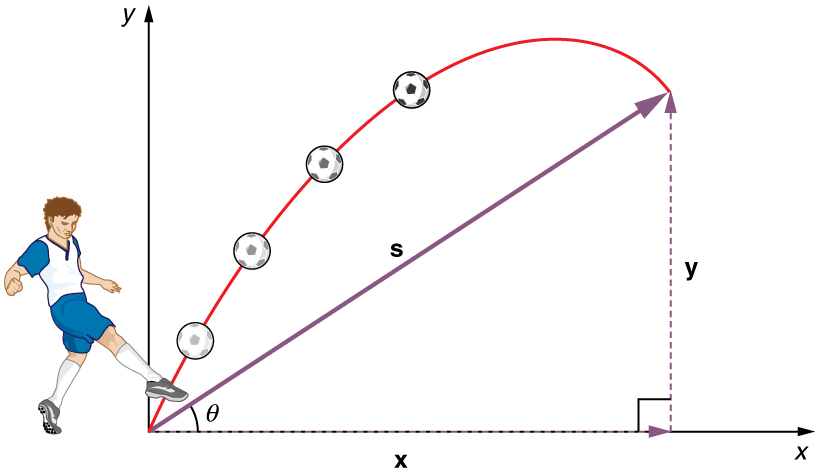
\includegraphics[width=0.5\textwidth]{figures/kick.jpeg}
\caption{\label{fig:1} A basic projectile motion trajectory.}
\end{figure}

\section{Chapter 4 - Forces}

\begin{enumerate}
\item A man pushes a crate of mass 50 kg.  The observed acceleration is 0.5 m s$^{-2}$.  What is the force the man generates on the crate?
\end{enumerate}

\end{document}
